\subsubsection{Nanocapsules}
\index{Winterhalter, Mathias}

\paragraph{Research Team}
%
Mathias Winterhalter (Professor), Yannic Ramaye (Postdoc), Dr. Helge Weingart (Project Manager), Tivadar Mach (PhD Student), Joana Gomes (PhD Student), Raghavendra Palankar (PhD Student), Que Tien Tran (PhD Student), Stefanie T�mmers (PhD Student)\\

Genomics and the recent development in molecular biology have brought a large variety 
of proteins, and notably enzymes useful for biotechnological applications in the area of 
biosensors, protein chips or biocatalysts. However, most proteins or enzymes are fragile 
and small conformational changes may reduce their activity. Therefore their stabilisation 
is required. One possibility to is to encapsulate the protein into nanometer sized vesicles 
to protect the enzyme from denaturation by proteolysis and dilution effects. Furthermore 
we may functionalise the capsule wall. Insertion of natural or engineered channel forming 
proteins all selective transport. Furthermore the outside of the capsule might be coated for 
stabilisation or with receptor peptides for targeting. 


\paragraph{Highlights}
%
A recent example from Rothemund demonstrated that encoding the DNA allows to create a large variety of 3-D structures in the nano to micrometer range. In collaboration with Dr. Fournier's group in Toulouse (IPBS-CNRS UMR 5089)  we use enzymes developed by molecular biologists as new promising tools to manipulate (synthesis, ligation or cutting) nucleic acids structure. Covalent grafting of oligonucleotides functionalizes the surface of liposomes which can be achieved with maleimid functionalised lipids. Subsequent addition of an enzyme called terminal deoxynucleotidyl transferase elongates the single stranded DNA. The elongated DNA hybridizes creating a random network. The short segments of double stranded DNA provides a substrate for the Klenow fragment of E. coli DNA polymerase which synthesizes a double strand DNA reinforcing the network. Alternate action of both enzymes leads to a three dimensional network anchored on the liposome surface. 

\begin{figure}[ht]
 \begin{center}
   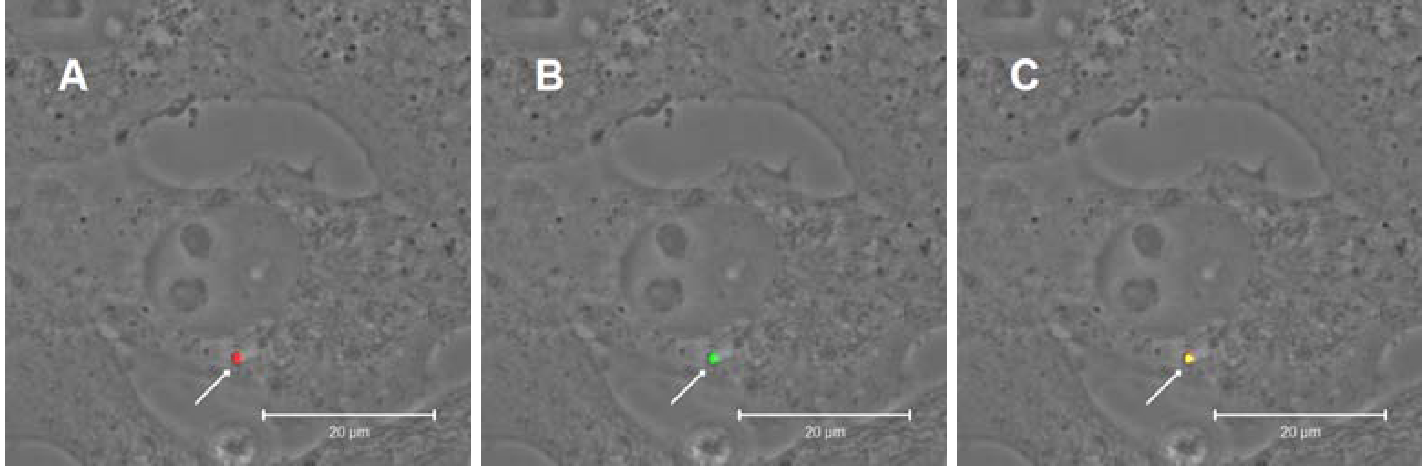
\includegraphics[width=\hsize]{Winterhalter/Winterhalter_fig2.pdf}
    \caption{Confocal Laser Scanning Microscopy (cLSM) images of uptake of liposome capsule by Vero cells in culture. The fig. A and B show fluorescence signals emitted from RhodamineB (RhoB) labelled lipids incorporated in the liposome bilayer and the PAH- fluorescein isothiocyanate (FITC) coated on the liposome respectively, and fig.C is a overlay of fig.A and fig.B confirming the co-localization of the two fluorescence signals coming from the liposome-capsule}
   \label{fig2:Winterhalter}
  \end{center}
\end{figure}

In collaboration with the group of S. Springer 
(IUB) and G.B. Sukhorukov (MPI-Golm) we transfer functionalised nanocapsules into 
living cells as in situ reporter. Two techniques are applied:
a) Electroporation is an established technique used to permeate temporarily cell 
membranes. For this, round cells are essential. This can be achieved by addition of 
trypsine to the CHO (Chinese Hamster Ovary, given from Prof. S. Springer, IUB) cells. 
For example, we succeeded to insert 1 $\mu$ (PSS/PAH-TRITC)4 labeled capsules provided 
by O. Kreft (MPI-Golm). Insertion was increased using smaller 200 nm polyelectrolyte 
coated liposomes. 



b) A second technique to introduce nanocapsules into the cells is by microinjection. A 
fluorescent microscope was equipped with an Eppendorf Femto Jet microinjection 
system connected to a micromanipulator InjectMan NI 2. Two kinds of adherent cells 
were used: CHO and VERO cells. Due to the size of the capillary used for the 
microinjection, only liposomes with a size below 400 nm can be use. 

Amphiphilic ABA triblock copolymers, like poly-(2-methyloxazoline)- block- 
poly- (dimethylsiloxan)- block- poly-(2-methyloxazoline) (PMOXA-PDMS-
PMOXA, provided by W. Meier, Basel), form vesicular structures or 
nanotubes. We we investigated the interaction of these ABA structures with 
liposomes by electron microscopy, fluorescence spectroscopy and differential 
scanning calorimetry. Our observations suggest a formation of homogenous 
mixed polymer-lipid structures whatever the method used to obtain the 
structure, film hydration, dispersion or detergent removal. When ABA 
polymersomes and liposomes are mixed, we observed monomer exchanges 
on a time scale of several minutes. This possibility to form mixed structures 
and to perform exchanges between pre-existing structures may allow to 
combine the properties of lipids and polymer structures such as stability or 
loading capacity. \newline \newline Mathias Winterhalter is also involved in ``Membrane Transport''.



\paragraph{Organization}
\begin{enumerate}
\item  We organized a summerschool on Biosensing: Faster smaller, smarter shop at IUB 
(28.7.-4.8.) with more than 100 participations from 12 countries. A second summerschool on Complex 
Materials from June 24th to Juli 1st. This summerschool included lectures and practical 
courses for about 50 participants in the field.  
\end{enumerate}


\paragraph{Collaborations}
Bremen Area Collaborations:
\begin{enumerate}
\item {\sl International University Bremen} \\ Prof. J. Fritz \\ Microfluidics for electrophysiology and liposome separation
\item {\sl International University Bremen} \\ Prof. U. Kleinekath�fer \\ Ion and antibiotics transport through membrane proteins 
\item {\sl International University Bremen} \\ Prof. S. Springer \\ Injection of engineered nanocapsules into cells for use as sensors
\item {\sl Uni Bremen, Chemie} \\ Prof D. Gabel 
\item {\sl Hochschule Bremen} \\ Prof. V. Hass 
\end{enumerate}
National \& International Collaborations:
\begin{enumerate}
\item R. Benz (University of W�rzburg) 
\item S.M. Bezrukov (NIH, Bethesda) 
\item G.B. Sukhorukov (MPI Berlin)
\item D. Fournier (University of Toulouse)
\item P. Faller (University of Toulouse)
\item P. Gameiro (University of Porto)
\item L. Movileanu (University of Syrakuse)
\item T. Heimburg (University of Copenhagen)
\end{enumerate}
 
\paragraph{Grants}
\begin{enumerate}
\item Funded by EU Training network, \emph{Molecular origin of antibiotic
    translocation}. This project is performed in collaboration with N. Fertig (M\"unchen),
  H. Vogel (Lausanne), J.M. Pages (Marseille), P. Gameiro (Porto), M. Page (Basel), PI
  M. Winterhalter. 

\item Funded by Volkswagen Foundation, \emph{Complex Materials: Cooperative Projects of
    the Natural, Engineering, and Biosciences}, Nanoengineered polymer capsules: Detection
  and manipulation for nanoreactors and controlled delivery. (I/80 051) in collaboration
  with G. B. Sukhorukov (coordinator, MPI  Potsdam), A. L. Rogach (LMU Munich) and
  W. J. Parak (LMU Munich)  

\item Funded by Volkwagen Foundation, \emph{Summerschool on Complex Materials}

\item Funded by German-french University, Summerschool on Biosening, faster, smaller,
  smarter. 

\item Funded by DAAD Exchange program with Porto

\item Funded by Eureka 3271 Nano to Bio (PI L. Levy, Nanobiotix, Paris; J.F. Hochepied,
  Ecole des Mines, Paris) 
\end{enumerate}


\nocite{Winterhalter1,Winterhalter2,Winterhalter3,Winterhalter4,Winterhalter5,Winterhalter6,Winterhalter7,Winterhalter8,Winterhalter9,Winterhalter10,Winterhalter11,Winterhalter12}